
\subsection{Suffix Arrays and Suffix Trees}


\begin{figure}
\centering
%\scalebox{0.9}{

\tikzstyle{leaf}=[draw=red!90,fill=red!40,rectangle,thick,minimum height=2.6ex,minimum width=2ex,inner sep=0pt]
\tikzstyle{internal}=[fill=black,circle,inner sep=0pt,minimum size=1ex]

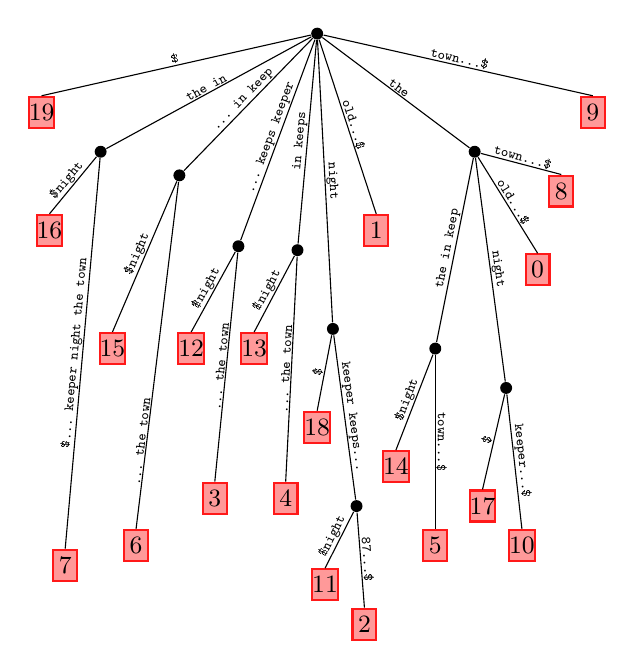
\begin{tikzpicture}
% \draw [help lines] (0,0) grid (7,7);
% \node at (0,0) {(0,0)};
% \node at (7,0) {(7,0)};
% \node at (0,7) {(0,7)};
% \node at (7,7) {(7,7)};

\node[internal] (root) at (3.5,7.5) {};

% children of the root
\node[leaf] (leaf-0) at (0,6.5) {\small$19$};
\node[internal] (root-subtree-1) at (0.75,6) {};
\node[internal] (root-subtree-2) at (1.75,5.7) {};
\node[internal] (root-subtree-3) at (2.5,4.8) {};
\node[internal] (root-subtree-4) at (3.25,4.75) {};
\node[internal] (root-subtree-5) at (3.7,3.75) {};
\node[leaf] (leaf-12) at (4.25,5) {\small$1$};
\node[internal] (root-subtree-6) at (5.5,6) {};
\node[leaf] (leaf-19) at (7,6.5) {\small$9$};

%children of root-subtree-1
\node[leaf] (leaf-1) at (0.1,5) {\small$16$};
\node[leaf] (leaf-2) at (0.3,0.75) {\small$7$};

%children of root-subtree-2
\node[leaf] (leaf-3) at (0.9,3.5) {\small$15$};
\node[leaf] (leaf-4) at (1.2,1) {\small$6$};

%children of root-subtree-3
\node[leaf] (leaf-5) at (1.9,3.5) {\small$12$};
\node[leaf] (leaf-6) at (2.2,1.6) {\small$3$};

%children of root-subtree-4
\node[leaf] (leaf-7) at (2.7,3.5) {\small$13$};
\node[leaf] (leaf-8) at (3.1,1.6) {\small$4$};

%children of root-subtree-5
\node[leaf] (leaf-9) at (3.5,2.5) {\small$18$};
\node[internal] (subtree-5-subtree-1) at (4,1.5) {};

%children of subtree-5-subtree-1
\node[leaf] (leaf-10) at (3.6,0.5) {\small$11$};
\node[leaf] (leaf-11) at (4.1,0) {\small$2$};

%children of root-subtree-6

\node[internal] (subtree-6-subtree-1) at (5,3.5) {};
\node[internal] (subtree-6-subtree-2) at (5.9,3) {};
\node[leaf] (leaf-17) at (6.3,4.5) {\small$0$};
\node[leaf] (leaf-18) at (6.6,5.5) {\small$8$};

%children of subtree-6-subtree-1
\node[leaf] (leaf-13) at (4.5,2) {\small$14$};
\node[leaf] (leaf-14) at (5,1) {\small$5$};

%children of subtree-6-subtree-2
\node[leaf] (leaf-15) at (5.6,1.5) {\small$17$};
\node[leaf] (leaf-16) at (6.1,1) {\small$10$};


% edge label mapping
% the 1       7
% old 2       6
% night 3     5
% keeper 4    3
% keeps 5     4
% keep 6      2
% in 7        1
% town 8      8


% edges from root to children
\draw (root) -- (leaf-0.north)  node [midway,above=-3pt,sloped] {\tiny \tt \$};
\draw (root) -- (root-subtree-1)  node [sloped,midway,above=-3pt] {\tiny \tt the in};
\draw (root) -- (root-subtree-2)  node [sloped,midway,above=-3pt] {\tiny \tt \ldots~in keep};
\draw (root) -- (root-subtree-3)  node [sloped,midway,above=-3pt] {\tiny \tt \ldots~keeps keeper};
\draw (root) -- (root-subtree-4)  node [sloped,midway,above=-3pt] {\tiny \tt in keeps};
\draw (root) -- (root-subtree-5)  node [sloped,midway,above=-3pt] {\tiny \tt night};
\draw (root) -- (leaf-12.north)  node [sloped,midway,above=-3pt] {\tiny \tt old\ldots\$};
\draw (root) -- (root-subtree-6)  node [sloped,midway,above=-3pt] {\tiny \tt the};
\draw (root) -- (leaf-19.north)  node [midway,above=-3pt,sloped] {\tiny \tt town\ldots\$};

% edges from root-subtree-1 to children
\draw (root-subtree-1) -- (leaf-1.north)  node [midway,above=-3pt,sloped] {\tiny \tt \$night};
\draw (root-subtree-1) -- (leaf-2.north)  node [midway,above=-3pt,sloped] {\tiny \tt \$\ldots~keeper night the town};

% edges from root-subtree-2 to children
\draw (root-subtree-2) -- (leaf-3.north)  node [midway,above=-3pt,sloped] {\tiny \tt \$night};
\draw (root-subtree-2) -- (leaf-4.north)  node [near end,above=-3pt,sloped] {\tiny \tt \ldots~the town};

% edges from root-subtree-3 to children
\draw (root-subtree-3) -- (leaf-5.north)  node [midway,above=-3pt,sloped] {\tiny \tt \$night};
\draw (root-subtree-3) -- (leaf-6.north)  node [midway,above=-3pt,sloped] {\tiny \tt \ldots~the town};

% edges from root-subtree-4 to children
\draw (root-subtree-4) -- (leaf-7.north)  node [midway,above=-3pt,sloped] {\tiny \tt \$night};
\draw (root-subtree-4) -- (leaf-8.north)  node [midway,above=-3pt,sloped] {\tiny \tt \ldots~the town};

% edges from root-subtree-5 to children
\draw (root-subtree-5) -- (leaf-9.north)  node [midway,above=-3pt,sloped] {\tiny \tt \$};
\draw (root-subtree-5) -- (subtree-5-subtree-1)  node [sloped,midway,above=-3pt] {\tiny \tt keeper keeps\ldots};

% edges from subtree-5-subtree-1 to children
\draw (subtree-5-subtree-1) -- (leaf-10.north)  node [midway,above=-3pt,sloped] {\tiny \tt \$night};
\draw (subtree-5-subtree-1) -- (leaf-11.north)  node [sloped,midway,above=-3pt] {\tiny \tt 87\ldots\$};


% edges from root-subtree-6 to children
\draw (root-subtree-6) -- (leaf-17.north)  node [sloped,midway,above=-3pt] {\tiny \tt old\ldots\$};
\draw (root-subtree-6) -- (leaf-18.north)  node [sloped,midway,above=-3pt] {\tiny \tt town\ldots\$};
\draw (root-subtree-6)  -- (subtree-6-subtree-1)  node [sloped,midway,above=-3pt] {\tiny \tt the in keep};
\draw (root-subtree-6)  -- (subtree-6-subtree-2)  node [sloped,midway,above=-3pt] {\tiny \tt night};

% edges from root-subtree-subtree-6-subtree-1 to children
\draw (subtree-6-subtree-1)  -- (leaf-13.north)  node [sloped,midway,above=-3pt] {\tiny \tt \$night};
\draw (subtree-6-subtree-1)  -- (leaf-14.north)  node [sloped,midway,above=-3pt] {\tiny \tt town\ldots\$};


% edges from root-subtree-subtree-6-subtree-2 to children
\draw (subtree-6-subtree-2)  -- (leaf-15.north)  node [sloped,midway,above=-3pt] {\tiny \tt \$};
\draw (subtree-6-subtree-2)  -- (leaf-16.north)  node [sloped,midway,above=-3pt] {\tiny \tt keeper\ldots\$};


\end{tikzpicture}
%}
\caption{Word-based Suffix Tree and Suffix Array for a sample the 
text.}
\label{fig-suffix-tree}
\end{figure}

Let {\col} be a string of size {\collen} drawn from an alphabet {\alphabet} of
size {\alphabetsize}. Let {$\col[i..n-1]$} be a {\it suffix} of {\col}.
The {\it suffix tree}~\cite{w-swat73} of {\col} is the compact labeled
tree of $n+1$ leaves where the root to leaf paths correspond to all suffixes of {\col\$},
where \$ is a terminating symbol not in {\alphabet}. The {\it path-label}
of each node $v$ corresponds to the concatenation of edge labels from the
root node to $v$. The {\it node depth} of $v$ corresponds to the number
of ancestors in the tree, whereas the {\it string depth} corresponds to the
length of the path-label. Searching for a pattern {\pattern} of 
size {\plen} in {\col} translates to finding the {\it locus} node $v$ closest to
the root such that {\pattern} is a prefix of the path-label of $v$ in $\Order{m}$ time.
Figure~\ref{fig-suffix-tree} shows a suffix tree over {\col=``\#the old night keeper 
keeps the keep in the town\# the night keeper keeps the keep in the night\#\$}''. 
The sample text is drawn from the word alphabet 
{\alphabet=\{the,old,night,keeper,keeps,keep,in,town,\#\}}. A suffix tree requires $\Order{n}$ space 
and can be constructed in $\Order{n}$ time~\cite{u-algo95}. The children
of each node in the suffix tree are lexicographically ordered by their edge labels.
The $i$-th smallest suffix in {\col} corresponds to the path-label of the $i$-th 
leaf. The starting postion of the suffix can be associated its corresponding
leaf in the tree as shown in Figure~\ref{fig-suffix-tree}. All 
occurrences of {\pattern} in {\col} can be retrieved by visiting all leaves
in the subtree of the locus of {\pattern}. For example, pattern ``the night'' occurs
at positions $12$ and $19$ in the sample text. We further refer the number of children
of a node $v$ as its {\it degree} and the number of leaves in the subtree rooted at $v$
as the {\it size} of $v$.

The {\it suffix array}~\cite{mm-jcomp93} of {\col} is an array $\SA[0\ldots n-1]$ such
that $\SA[i]$ corresponds to the starting position of the $i$-th smallest suffix
in {\col} or the $i$-th leaf in the suffix tree of {\col}. The suffix array requires
$n \log n$ bits of space and can also be constructed in $\Order{n}$ time~\cite{ksb-jacm06}.
Using only the suffix array and the text, pattern search can be performed using binary search
in $\Order{m \log n}$ time.
In practice, suffix arrays use $4-8n$ bytes of space whereas the most efficient
suffix tree implementations require at least $20n$ bytes of space~\cite{k-spe99} which
are both much larger than {\col} and prohibit the use of these structures for all but
small data sets.

\subsection{Compressed Suffix Structures}

WT, nested brackets CST, rank/select etc. Wiener links even?
